\documentclass{scsSimAUDPaperFormat}

\usepackage[utf8]{inputenc}
 
\usepackage{listings}
\usepackage{xcolor}
\pagenumbering{arabic}
\definecolor{codegreen}{rgb}{0,0.6,0}
\definecolor{codegray}{rgb}{0.5,0.5,0.5}
\definecolor{codepurple}{rgb}{0.58,0,0.82}
\definecolor{backcolour}{rgb}{1.0, 1.0, 1.0}
 
\lstdefinestyle{mystyle}{
    backgroundcolor=\color{backcolour},   
    commentstyle=\color{codegreen},
    keywordstyle=\color{magenta},
    numberstyle=\tiny\color{codegray},
    stringstyle=\color{codepurple},
    basicstyle=\ttfamily\small,
    breakatwhitespace=false,         
    breaklines=true,                 
    captionpos=b,                    
    keepspaces=true,                 
    numbers=left,                    
    numbersep=5pt,                  
    showspaces=false,                
    showstringspaces=false,
    showtabs=false,                  
    tabsize=4
}
 

% Beginning of preable.
% Ensure that the copyright notice matches the conference/symposium.
\copyrightnotice{
	SimAUD 2020 May 25-27 Vienna, Austria
	
	\copyright\,2020 Society for Modeling \& Simulation International (SCS)
}
% Load basic packages
\usepackage{balance}		% to better equalize the last page
\usepackage{graphics}		% for EPS, load graphicx instead
\usepackage{times}			% comment if you want LaTeX's default font
\usepackage{url}			% llt: nicely formatted URLs
\usepackage{dblfloatfix}	% allow placement of a page-width figure at top or bottom of page
% llt: Define a global style for URLs, rather that the default one

\usepackage{lipsum}  
\usepackage{soul}
\makeatletter
\def\url@leostyle{%
  \@ifundefined{selectfont}{\def\UrlFont{\sf}}{\def\UrlFont{\small\bf\ttfamily}}}
\makeatother
\urlstyle{leo}

% To make various LaTeX processors do the right thing with page size.
\def\pprw{8.5in}
\def\pprh{11in}
\special{papersize=\pprw,\pprh}
\setlength{\paperwidth}{\pprw}
\setlength{\paperheight}{\pprh}
\setlength{\pdfpagewidth}{\pprw}
\setlength{\pdfpageheight}{\pprh}

% Make sure hyperref comes last of your loaded packages,
% to give it a fighting chance of not being over-written,
% since its job is to redefine many LaTeX commands.
\usepackage[pdftex]{hyperref}
\hypersetup{
pdftitle={SCS Conference Proceedings Format},
pdfauthor={LaTeX},
pdfkeywords={SCS, proceedings, archival format},
bookmarksnumbered,
pdfstartview={FitH},
colorlinks,
citecolor=blue,
filecolor=black,
linkcolor=blue,
urlcolor=blue,
breaklinks=true,
colorlinks=true,
}
% \hypersetup{
%     colorlinks=true,
%     linkcolor=blue,
%     filecolor=magenta,      
%     urlcolor=cyan,
% }
% create a shortcut to typeset table headings
\newcommand\tabhead[1]{\small\textbf{#1}}

% create an affilitation superscript
\newcommand{\affiliation}[1]{\ensuremath{^{\textrm{#1}}}}

% End of preamble. Here comes the document.
% \tolerance=1
% \emergencystretch=\maxdimen
% \hyphenpenalty=10000
% \hbadness=10000
\begin{document}
% \title{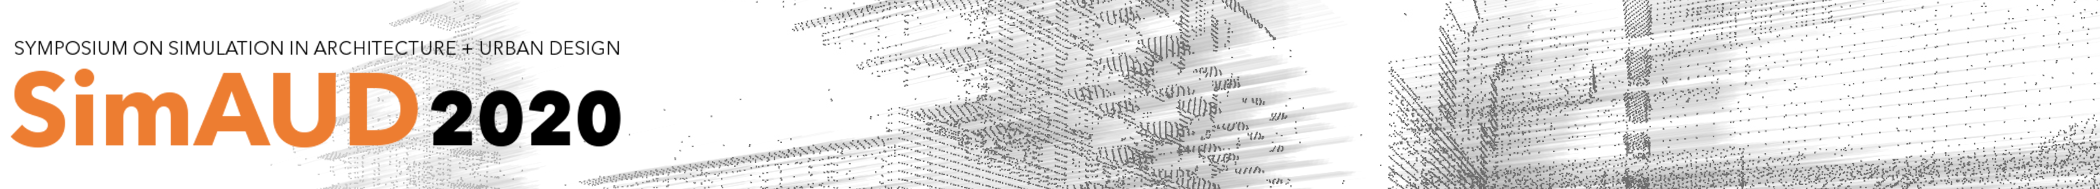
\includegraphics[width=1.0\textwidth]{SimAUDLogo.png}\\\quad\\BuildFit: A Model-Veiw-Controller (MVC) Open Platform for Building-Lifecycle Data Analysis and Energy Modelling }

\title{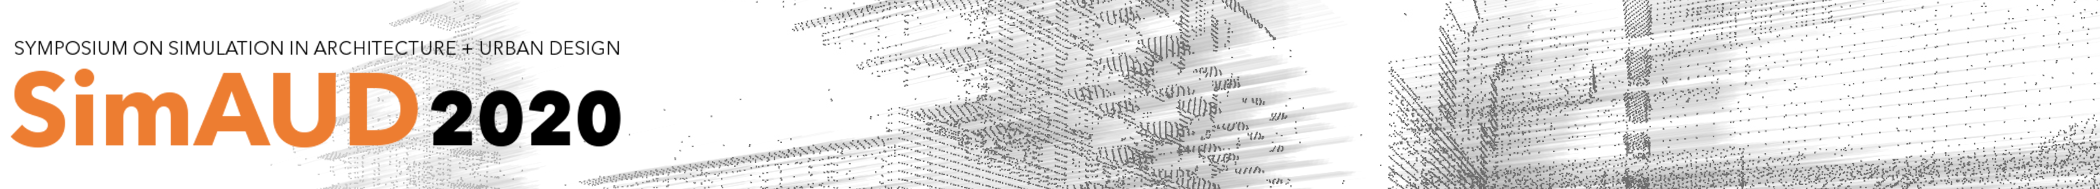
\includegraphics[width=1.0\textwidth]{SimAUDLogo.png}\\\quad\\A Three-Tier Architecture Visual-Programming Platform for Building-Lifecycle Data Management }

% Replace "UniversityA", "CompanyA", "UniversityB" with institution-specific abbreviations.
\def\UniversityA{\affiliation{1}} 
\def\CompanyA{\affiliation{2}}
\def\UniversityB{\affiliation{3}}

\author{
% 	Author1\UniversityA
% 	,
% 	Author2\UniversityA
% 	,
% 	Author3\UniversityA
% 	\\
% 	\\
% \affaddr{\UniversityA}{Department, School, University, Country, zipcode.}\\
}


\author{
	Mahmoud M. Abdelrahman\UniversityA
	,
	Sicheng Zhan\UniversityA
	,
	Adrian Chong\UniversityA
	\\
{\\^1 \textbf{\large Department of Building, School of Design and Environment,}\\The National University of Singapore, 4 Architecture Drive, Singapore 117566.}\\
}

\maketitle

\begin{abstract}
	In this paper, we present a platform that integrates three main aspects in the building industry: 1) Building data from both IoT devices and Building Management System (BMS), 2) Building Energy modeling and simulation engine, and 3)Data analysis and optimization libraries. All of which are combined in a three-tier architecture cloud platform. The platform aims to provide useful representations of the data to different stakeholders. We defined three main types of stakeholders. Each stakeholder uses the platform differently: (1) End-use programmers, who use visual programming and textual programming interfaces to perform computational tasks, (2) Dashboard viewers who are interested in viewing insightful real-time data about performance in the form of charts and diagrams, and (3) Data feedback inputters such as occupants to give feedback or fill questionnaires. The three-tier architecture enables the spatial and physical separation of the databases, the computational engines, and the user-interfaces. This separation resulted in some advantages such as flexibility, scalability (horizontal and vertical), reusability, and latency reduction. \hl{Currently, the platform is in the final stage of development. The following stage includes community testing and user experience enhancement.}
\end{abstract}

\keywords{
	three-tier architecture;
	n-tier architecture;
	Building Energy Modelling;
	BEM;
	building lifecycle;
	actors;
	presentation layer;
	application layer;
	data layer
}

% ACM Classification Keywords
\category{I.6.1}{SIMULATION AND MODELING}
Computing methodologies ~ Model development and analysis - 
Software and its engineering ~ Visual languages
% See: \url{http://www.acm.org/about/class/1998/} for more information and the full list of ACM classifiers and descriptors.
% \textcolor{red}{Optional section to be included in your final version, but strongly encouraged.}
\section{Introduction}
The building sector has witnessed immense development recently in the way by which building systems are managed \cite{ WongIntelligentReview}. This development aimed at alleviating the significant environmental impact of this sector (30\% of the world energy consumption and a third of the associated CO2 emissions \cite{Iea2013TrackingMinisterial}). Decreasing this impact could be achieved by better controlling the resources \cite{Allcott2010BehaviorPolicy}; providing sustainable, and more efficient solutions \cite{Zhang2019WholeLearning}; developing a better understanding of different deterministic and stochastic aspects of the built environment \cite{Brohus2012QuantificationApproach,ReviewsStochasticReview, USDepartmentofEnergy2018TechnologyReport, Chong2015UncertaintyApproach}. In addition, making better decisions based on mining ground-truth data (black-box approach)\cite{Molina-Solana2017DataReview}, physics-based simulation models (white-box approach)\cite{TardioliDataLevel,Molina-Solana2017DataReview} or both of them (gray-box approach)\cite{Zhang2019WholeLearning}. 

The emergence of the Internet of Things (IoT) devices has enabled a massive amount of data, which posed some challenges. The data collected during the last two decades exceeded that which has ever been collected in history\cite{Ramaswamy2015InternetReview}. Two significant challenges, other than the availability of data, are to be addressed. On the one hand, managing this big data: transferring, storing, preprocessing, wrangling and mining, optimization, and control in a robust cyber-infrastructure. This lead to cloud computing or ubiquitous computing, that is, computing data in place, without paying much effort in transferring data to local storage/processing machines using scalable storage and computational power on demand maintained by professionals \cite{MellTheTechnology,Bhardwaj2010Cloud,Dillon2010CloudChallenges}. On the other hand, delivering useful information to different stakeholders based on their use is yet another challenge.

% Making use of this massive amount of data from the built environment requires 
"Data is not information; data must be presented in a usable form before it becomes information" \cite[p.134]{Reen1996UsabilityFramework}. Raw data from the built environment varies in its degree of usefulness to different stakeholders (actors). "Usability" is different for different stakeholders. For instance, A Building Energy Modeller (BEM) requires data such as Green Building eXtensible Markup Language (gbXML) \cite{GreenBuildingXMLgbXMLSchema2019GbXMLSchema}, schedules of operations, set-points, number of occupants,etc.. At the same time, a Facility Manager (FM) would be more interested in reducing maintenance costs by fault detection and diagnostics (FDD)\cite{Zibion2018DevelopmentInformation} algorithms and dashboards. This difference in uses requires users with proper domain knowledge alongside with programming or procedural thinking skills for automating, prototyping, analyzing, building work-flows using the big data and IoT sensors. At the same time, they do not need to be professional programmers, but rather End-use programmers.

The term \textit{End-use programmer} (or Novice developer) first introduced by \cite{Nardi1993AComputing} is used to describe non-professionals without programming and code structures knowledge \cite{InteractionDesignFoundation2014End-UserEd.}. Most programs today are written by novice programmers \cite{Rothermel2011TheEngineering} who use spreadsheets, writing add-ons/plugins to support their work or add functionality to the software, running MATLAB simulations \cite{Mathworks2016MATLABSimulink}, writing python codes, or IPython notebooks \cite{ScaffidiEstimatingProgrammers}. The main difference between the end-user developer and the professional developer is the goal of the development. The former writes a program focusing on getting tasks done without paying attention to debugging, unit-testing, or re-usability. However, the latter develops, maintain, debug, and test a robust software for others to use\cite{LiebermanEnd-userDevelopment}. End-use development mostly involves modifying or extending a software artifact (known as programming by example, or programming by demonstration). For example, \textit{Extended annotation or parameterization}: whereas a user can define a new functionality by selecting a readily developed set of functions by other users and stored in shared repositories \cite{Lieberman2006End-UserParadigm}. To make this task handy to end-use programmers, a proper programming notation should be utilized.

\textit{Programming notation} is the way by which a programming language is used to represent the state of the world\cite{Green2004InstructionsDescriptions}). The selection of the proper programming notation (e.g., textual, diagrammatic, or gesture-based) to describe the problem is a trade-off between several evaluation criteria\cite{Green2004InstructionsDescriptions}. This trade-off should lead non-specialist to find the programming environment easy-to-use and easy-to-understand. 

A large body of studies have addressed some difficulties related to the everyday programming tasks such as, but not limited to, code navigation \cite{DeLine2006CodeCode}, and hidden dependencies. A study conducted by Bragdon et al. \cite{Bragdon2010CodeMaintenance} that uses visual programming 2d spatially connected blocks of codes where it is possible to track each function in the form of bubble showed that visual programming significantly improve code understanding with less code navigation time.

Visual Programming Language (VPL), also known as box-and-wire programming or data-flow programming utilizes user-friendly graphical elements to display the flow of data between different components (Figure \ref{fig:vpl_example}). To date, there has been little agreement on the superiority of visual programming languages (VPLs) over the textual programming languages (TPLs). Green et.al. \cite{Green1991ComprehensibilityConjecture} and Moher et.al. \cite{Moher1993ComparingPrograms} adopted this stance. However, \cite{MENZIES2002EVALUATIONLANGUAGES} argued that VPLs could be significantly useful in motivating beginners to learn to program as they are informative in the sense of spatial reasoning and ideas generation. However, he argued that those advantages are not generalized and should not be isolated from the task being studied. Also, TPL is more productive in terms of large-scale and complex software development tasks. There is no conclusive evidence of the superiority of one over the other. Thus, a hybrid VPL/TPL is proven to be suitable amongst users. Many software enables this type of scripting which gained wide popularity such as Rhinoceros VPL Grasshopper\cite{Bachman2017Grasshopper:3D,McNeel2010GrasshopperRhino} whose user-community extended its limits by contributing to developing TPL based functions amongst others for building and urban simulation \cite{RoudsariLadybug:Design, PeronatoIntegratingCitySim,Koltsova2011ComponentsGeometry}, daylight analysis \cite{Jakubiec2011DIVAEnergyPlus,Lagios2010AnimatedDaysim}, Machine learning\cite{Abdelrahman2017EnhancingLanguage,AbdelRahman2017GH_CPython:Grasshopper,Abdelrahman2019ANT:Development}.

This research addresses two primary problems:
\begin{enumerate}
    \item Managing buildings' big data requires flexibility and scalability.
    %Maybe a better problem the VP addresses is the ability to connect data to mode
    \item Different users use data differently.
\end{enumerate} 

\begin{figure}
\centering
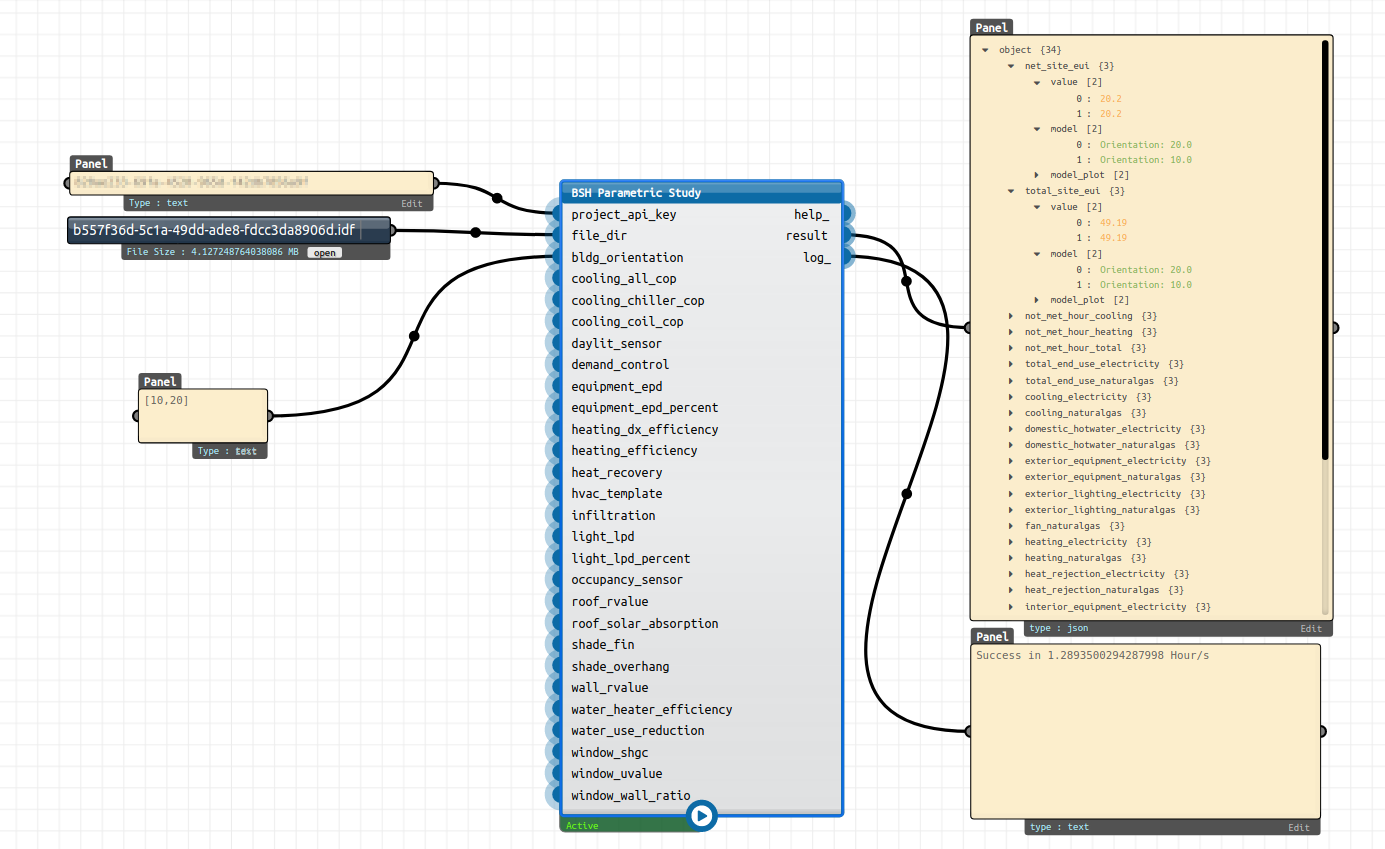
\includegraphics[width=0.9\columnwidth]{imgs/vpl_example.png}
\caption{A screenshot from our platform indicating a parametric simulation process on the cloud using (BuildSimHub). The figure is an example of Visual programming Language (also known as box-and-wire programming notation, and data-flow programming) where blocks of code functions are encapsulated in the boxes (known as components), while data flows from one or more component output variable to other component input variable. A component can hold as many inputs as needed, while the code behind each component follows a specific schema. Some components are used only as input components such as "file, numerical, panel" and some components work as output visualizations such as "panel, 3d visualization canvas, plotting components .."}
\label{fig:vpl_example}
\end{figure}
We introduce a Three-tier architecture web platform as a resolution to these problems. The objectives of this research are: (1) Making IoT data from the built environment useful to different stakeholders, (2) An Open platform for developing and sharing different models amongst end-use programmers. (3) Provide flexibility and scalability by separating the platform into three distributed layers. The rest of the paper is structured as follows: In section \ref{section1}, we explain the three-tier architecture. The components of the three-tier architecture are explained in details in the subsequent sections \ref{section3} (Actors), \ref{sec:presentationLayer} (Presentation Layer), \ref{sec:applicationlayer} (Application Layer), and \ref{sec:datalayer} (Data Layer).

\section{Three-Tier Architecture}
\label{section1}
\textit{Three-tier architecture} is a client-server software architecture pattern that has several potentials in distribution applications \cite{Booch2008Object-orientedEdition}. The key aspect of this architecture is that it enables the reusability of program building blocks (also referred to as components) such as sharing software components at run time, replicating the same component, controlled adaptation of code, or independent adaptation of components \cite{Taylor1998ThePerspective,Wijegunaratne1998DistributedEngineering}. This pattern consists of three functionally separated layers \cite{Schuldt2017Multi-tierArchitecture} (Figure \ref{fig:figure1}), those are: \textbf{1) Presentation layer} (the client-side), \textbf{2) Application layer} (also known as business logic, controllers and process management layer), and \textbf{3) Data layer} (also known as data storage). The presentation layer constitutes the user-interface side of the application. All human-computer interactions (HCI) happen on this layer. On the other side, the Business logic layer consists of the core engine where component functions that carry out the workload by receiving requests from the presentation layer get the relevant data from the Data layer and process this data then, sends back the response to the presentation layer. Finally, the Data layer consists of data querying (acquire from a data source), storage (stored in the relational database on a local server), and accessing (feed to the user). Each of these three tires is discussed in detail in the subsequent sections. A summarized workflow is illustrated in figure \ref{fig:structure}. 

\begin{figure}
\centering
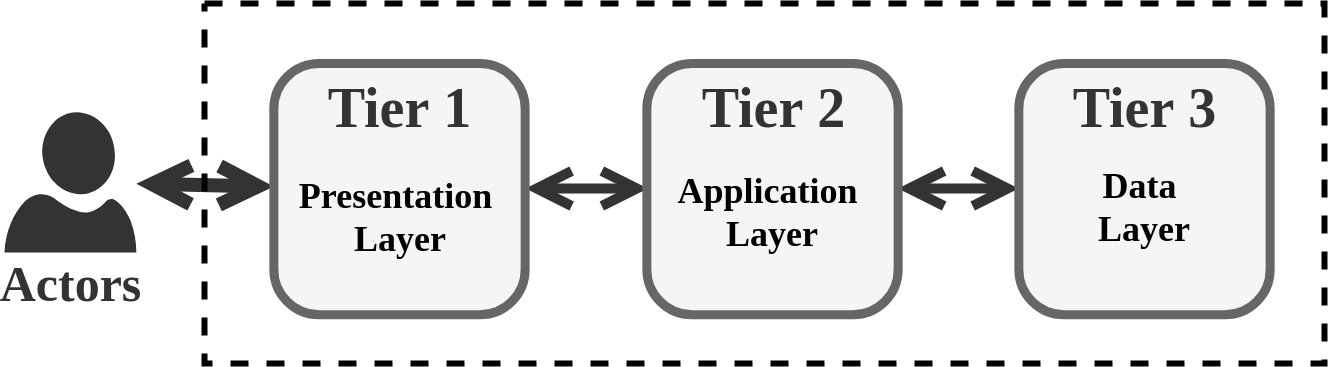
\includegraphics[width=0.9\columnwidth]{imgs/three_tier_architecture_summary.png}
\caption{Three-tier architecture structure of the platform}
\label{fig:figure1}
\end{figure}

\begin{figure*}[ht]
\centering
\includegraphics[width=0.8\linewidth]{imgs/allStructure.png}
\caption{This figure shows the flow of data within the three tiers: (1) The actor interact with the presentation layer three ways: programming, viewing dashboards, or giving feedback; (2)The user interaction results in sending requests to the application layer to be processed; (3)The application layer starts processing inputs and relevant functions; (4) If there is any required data from the databases, a QUERY is sent to the data layer; (5) then, the data layer respond with the corresponding data from different databases (6,7); (8) The application layer then runs the required components using the distributed engines; (9) The output of step (7) is responded back to the presentation layer along with the logs/errors in JSON format. higher resolution image can be downloaded \href{https://user-images.githubusercontent.com/6969514/72152397-cee71700-33e5-11ea-9108-c6823d2be504.png}{here}
}
\label{fig:structure}
\end{figure*}

Advantages of using three-tier architecture \cite{Furht2010HandbookComputing}:
\begin{enumerate}
    \item Reusability: The use of a modular component-function system enables many users/developers to contribute to the development. This contribution is shared in a public repository to be reusable by other users with small or no change
    \item Scalability (both horizontally and vertically) is another essential feature of using three-tier architecture because of using distributed servers as well as because of its separation nature. Horizontal Scalability is achieved by adding more nodes of the same types where required. While the Vertical Scalability is achieved by adding more resources to a host node on demand. On the other hand, separating different tiers allows scaling each one independently depending on the needs at any given time. 
    % The more the new users, nodes, or components are added, the more the resources are scaled out horizontally (adding new resources of the same type) to fit the load. 
    \item Flexibility: As server nodes that are used in the application layer could be developed, configured and tested separately without affecting any of the other layers, and then it could be added to the system on demand. Readily PaaS (Platform as a Service) is used to maintain consistency and Scalability. 
    \item Latency reduction: As the nodes are distributed on data centers that are spatially close to the end-user as possible. This is basically handled by adopting open PaaS (Platform as a Service) where the infrastructure complexity of servers are maintained and optimized by professionals. 
    \item Anytime data processing regardless of the user's connection speed. The connection between the application layer and the data layer is separated from the presentation layer, reducing the bandwidth load on the user's side.
    
\end{enumerate}

\section{actors}
\label{section3}
We use the term "Actor" to refer to different users/stakeholders within the built environment. "Usability" is the critical factor in obtaining "information" from data. Data obtained from the built environment does not hold equal usefulness for all stakeholders. Furthermore, in its raw format, IoT data consists of many problems, including noise, missing data, non-valid data, ill-labeled data points, duplicates, and non-standardized IoT representation. These problems should be dealt with before delivering this data to non-expert users. We define some actors or stakeholders who are involved in the building's life cycle energy modeling and data analysis and their corresponding data usage based on a systematic review conducted by Zou et.al \cite{Zou2018ReviewPerspectives} of 10 years publications till 2017 and  using Natural language processing (NLP) \cite{Abdelrahman2020BuildingWord-Embeddings}.

% \begin{figure}[h]
% \centering
% 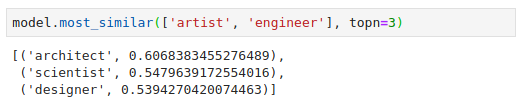
\includegraphics[width=0.9\columnwidth]{imgs/sim_art_eng.png}
% \caption{Using word embeddings, it is possible to do arithmetic vector operations on words, e.g. 'artist' + 'engineer' $\sim$ 'architect','designer', and - not surprisingly - 'scientist'.}
% \label{reasonablemeaining}
% \end{figure}

% \begin{figure}[h]
% \centering
% 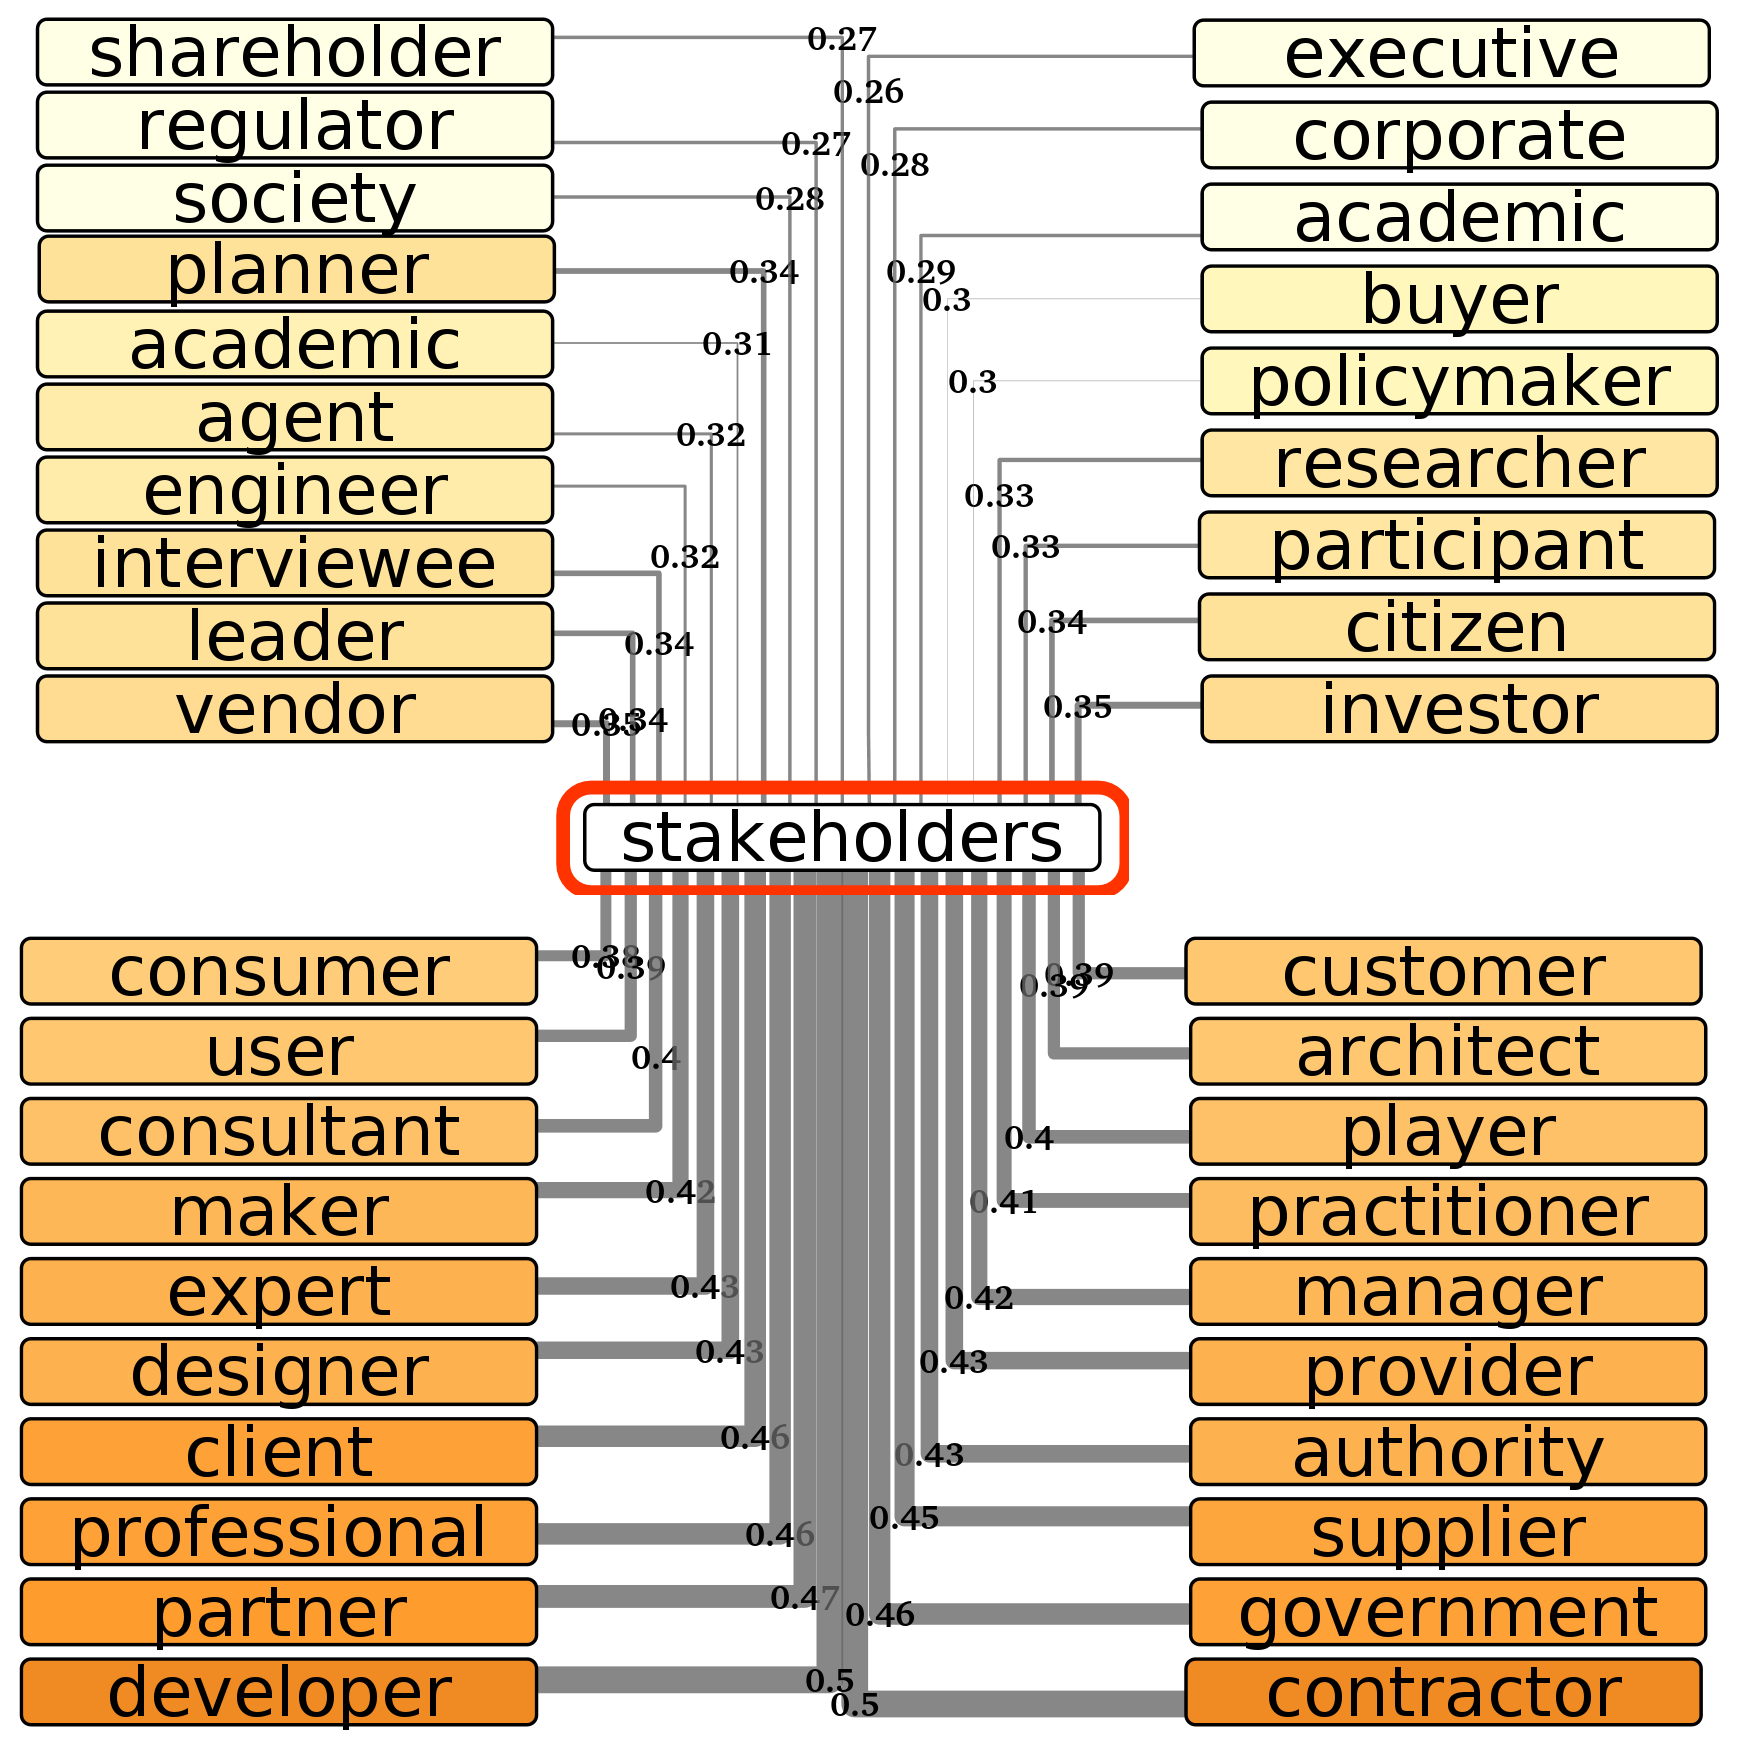
\includegraphics[width=0.8\columnwidth]{imgs/stakeholders.png}
% \caption{A list of \textit{filtered actors} (They are manually filtered because the original list consists of many words that do not represent actors.) words similar to the word "Stakeholder" are extracted from NLP mining building-related articles. The darker the color, the more the similarity index. The thickness of the edge (as well as the label on the edge) show the similarity index (i.e., this word appears more frequent in the context where "stakeholder" appears) \cite{Abdelrahman2020BuildingWord-Embeddings}.}

% \label{fig:figure4}
% \end{figure}

% \begin{figure}[h]
% \centering
% 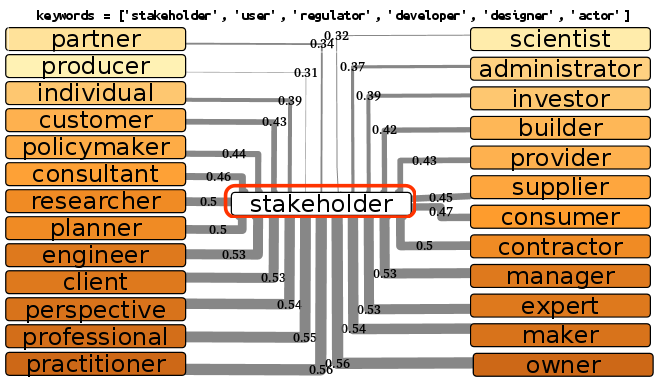
\includegraphics[width=0.8\columnwidth]{imgs/stakeholder3.png}
% \caption{ After narrowing down the scope of similarity search (by aggregating more keywords related to 'stakeholders.') 
% \cite{Abdelrahman2020BuildingWord-Embeddings}
% . The darkness of the color means a higher similarity, and the thickness of the edge represents a higher similarity as well.}
% \label{fig:figure5}
% \end{figure}

Then, we identified three main data-related actions, namely, \textbf{End-use programming}, \textbf{Data monitoring}, and \textbf{Data input}. Different stakeholders are clustered based on these three activities (Figure \ref{fig:figure6}). Then, these activities are reflected in the presentation layer \textit{(explained in section \ref{sec:presentationLayer})}  as three major components: 1) Hybrid VPL/TPL interface, 2) Interactive, shareable, embedded dashboards, and 3) Shareable, embedded forms. The interface of the platform is shown in figure \ref{fig:platformInterface}.

\begin{figure}[h]
\centering
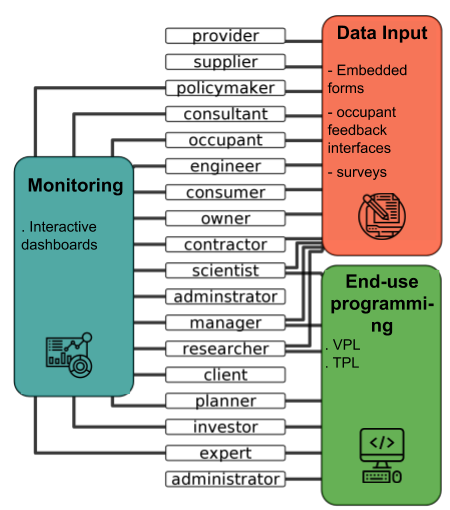
\includegraphics[width=0.8\columnwidth]{imgs/presentation_layer.png}
\caption{Actors are functionally clustered into three categories: Data monitoring, Data input, and End-use programming. Those categories constitute the Presentation layer.}
\label{fig:figure6}
\end{figure}

\section{Presentation Layer}
\label{sec:presentationLayer}
The presentation layer acts as the interface for the users. Each new project has a unique global unique identification (GUID), which is stored on the data layer and could be called using its GUID. Three main functions used in the presentation layer: (1) Visual/Textual programming interface, (2) dashboards, and (3) forms are used.

\begin{figure*}[h]
\centering
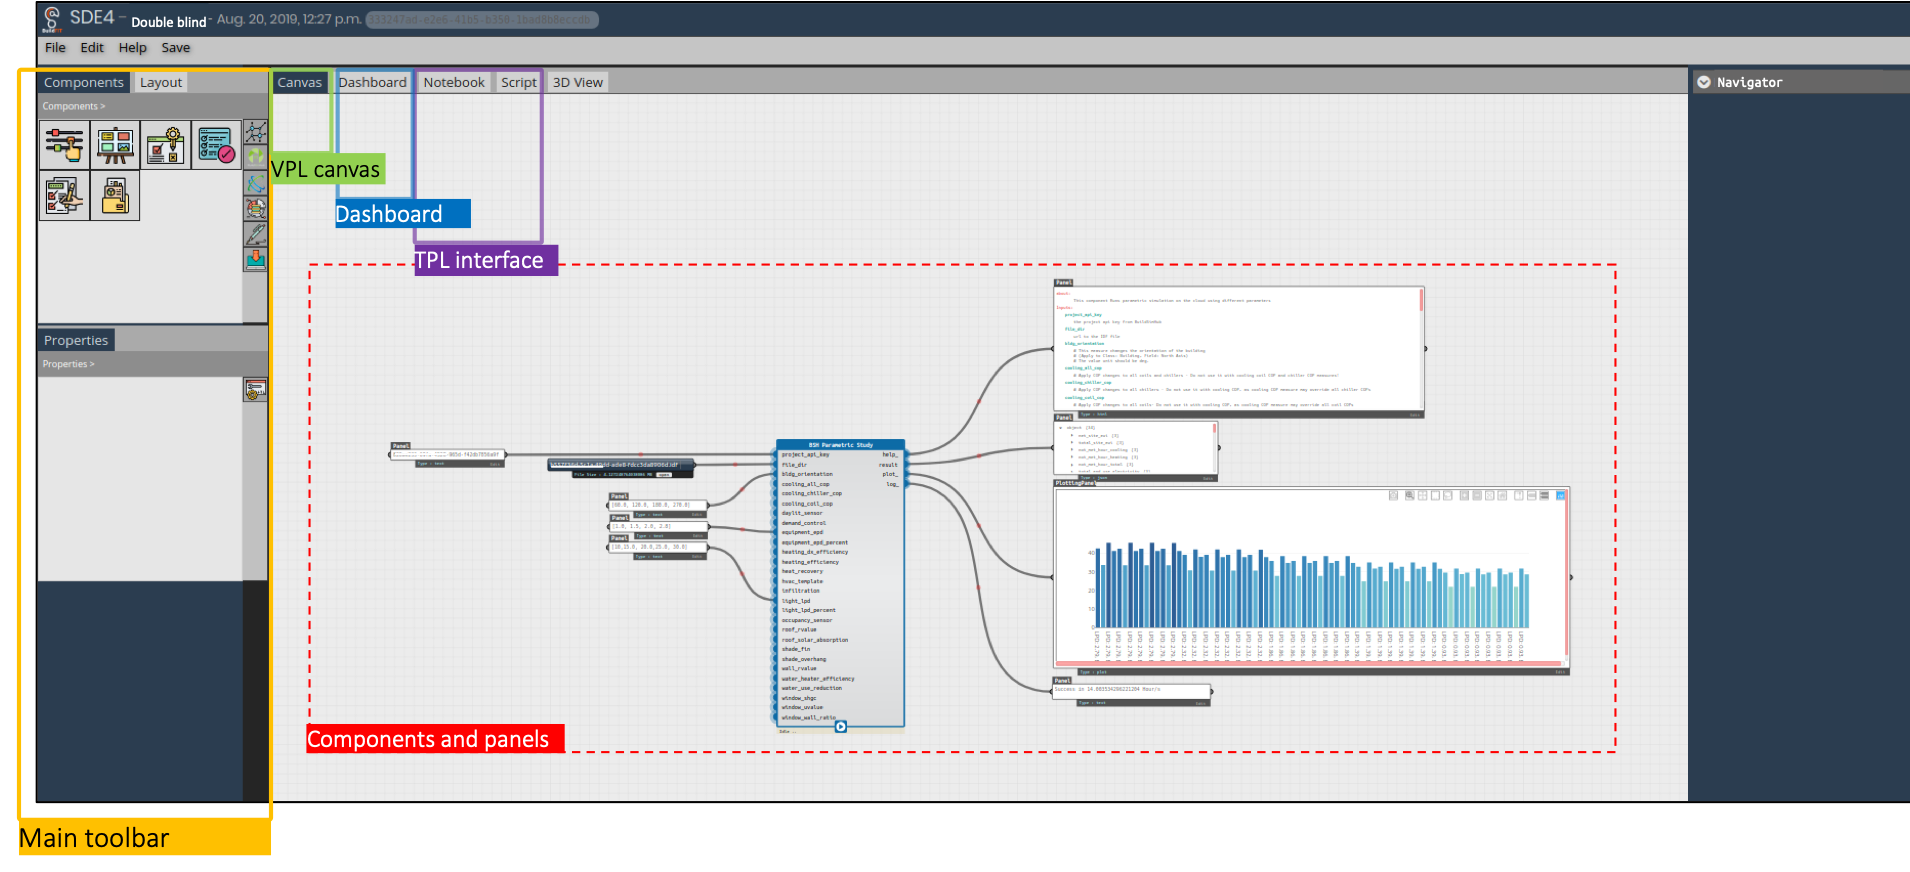
\includegraphics[width=\linewidth]{imgs/platform_interface.png}
\caption{The main interface functions}
\label{fig:platformInterface}
\end{figure*}

\subsection{VPL/TPL interface}
Both the visual and the textual programming interface use two main languages: Python and JavaScript. However, the selection of which is based on the complexity of the task and the response time required. For example: if the component function requires a real-time reaction, then it is more suitable to use a JavaScript component/script. We refer to the component in this case as \textit{"Shallow Function"}. While if the function requires heavy calculation such as Machine Learning (ML), or Energy Simulation (ES), then Python-based components/scripts are used and are referred to as \textit{"Deep Functions"}. Examples are shown in figure \ref{fig:deep-shallow}. 

\begin{figure}[h]
\centering
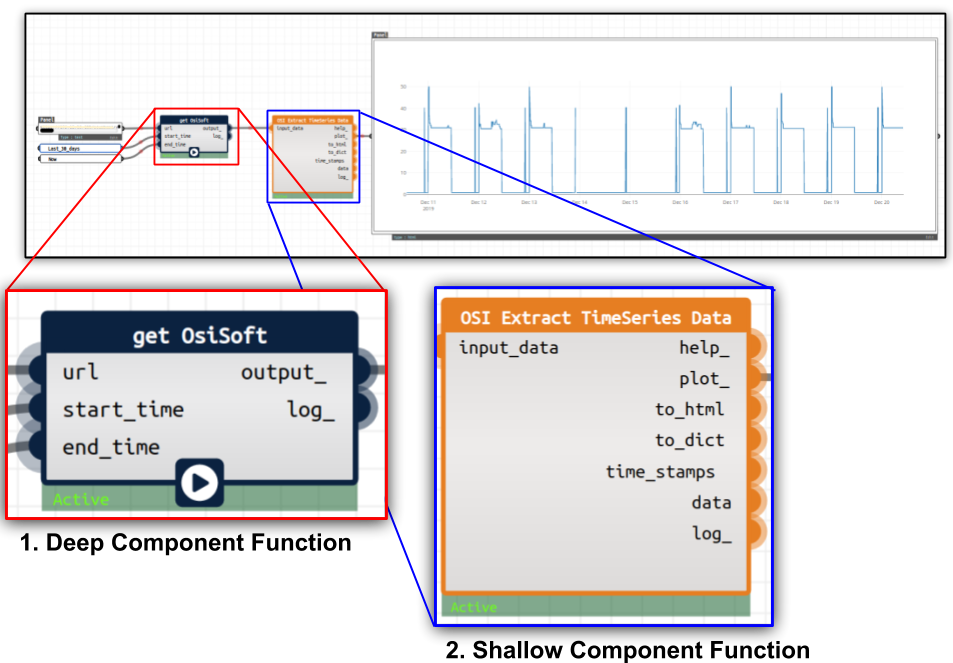
\includegraphics[width=\columnwidth]{imgs/shallow_deep.png}
\caption{Two examples of Shallow and Deep functions. 1. The deep function is Python-based, and hosted on the application layer, the "play button" on the bottom of the component must be clicked to run the deep function. 2. The shallow function is JavaScript based and is hosted on the front-end. However, all the shallow functions are stored in the data layer and follow specific schema. The shallow functions are used to implement real-time actions, such as arithmetic operations, and JavaScript Object Notation (JSON) parsing. In this figure, the deep function on the left uses OSISoft Python API to request time-series data from the data layer and outputs it as a JSON object. Then, the shallow component on the right parses the JSON object and converts it into different formats, including plotting.}
\label{fig:deep-shallow}
\end{figure}

Each component must follow specific abstraction schema that defines its structure and relationships as well as its types. Mainly, it consists of inputs, the function body, and outputs. However, other information must be provided when defining a new component e.g., The \texttt{dataflowType}: either shallow or deep, the component \texttt{type}: numeric, panel, optionList, ListItem, Plot, Generic, etc., the \texttt{category} where this component falls into, and other supplementary features such as the color, documentation, and license. 

\begin{figure}[h]
\centering
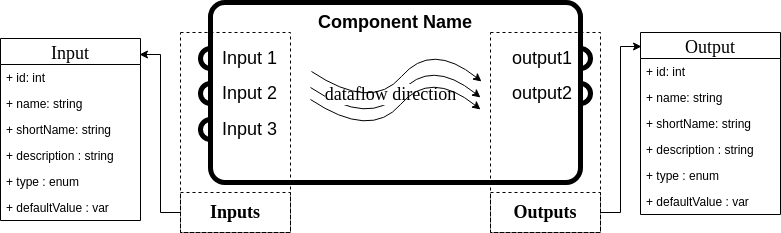
\includegraphics[width=\columnwidth]{imgs/component.png}
\caption{The data flows within components from left to the right. Each input of the component either carries a default value or receive value from other component's output, this value is stored in the input until the component runs, then the input variables are processed by calling the corresponding function. After the function is called, the return output of the function is stored back into the output of the component unless this output is connected to other component's input, it runs the other component automatically.}
\label{fig:component}
\end{figure}

Each component has a unique GUID on a project level. This GUID is used to trigger the component and call its inputs and outputs using the TPL panels. For example: the deep component (Figure \ref{fig:deep-shallow}) has a GUID : \texttt{'c56ad1cf-47ea-4fe3-805b-84d104ecff8b'} could be triggered using the Python API . This allows the end-use programmer to extend the functionality of the components by running blocks of codes either before running the component (i.e. doing preprocessing to the inputs) or after running the component (i.e. doing post-processing to the outputs) using the functions \texttt{before(callback)} and \texttt{after(callback)} as shown in listing \ref{lst:trigger_vpl} and figure \ref{fig:tpl_interface}.

\begin{lstlisting}[style=mystyle,
language=Python,
caption={Triggering a VPL component using TPL Pyton interface},
label={lst:trigger_vpl}]
import buildFit as bf
import json

component = bf.getComponent.by_guid("c56ad1cf-47ea-4fe3-805b-84d104ecff8b")
if component.inputs[0] == None:
    compoent.inputs[0] = "http://google.com"

def preprocessInputs(input1):
    '''This function is applied to the input before running the component'''
    return input1

def postprocessOutputs(output1):
    '''This function is applied to the output after running the component'''
    return json.parse(output1)

inp1 = component.before(preprocessInputs, component.inputs[0])
out1 = component.after(postprocessOutputs, component.outputs[0])
\end{lstlisting}

\begin{figure}[h]
\centering
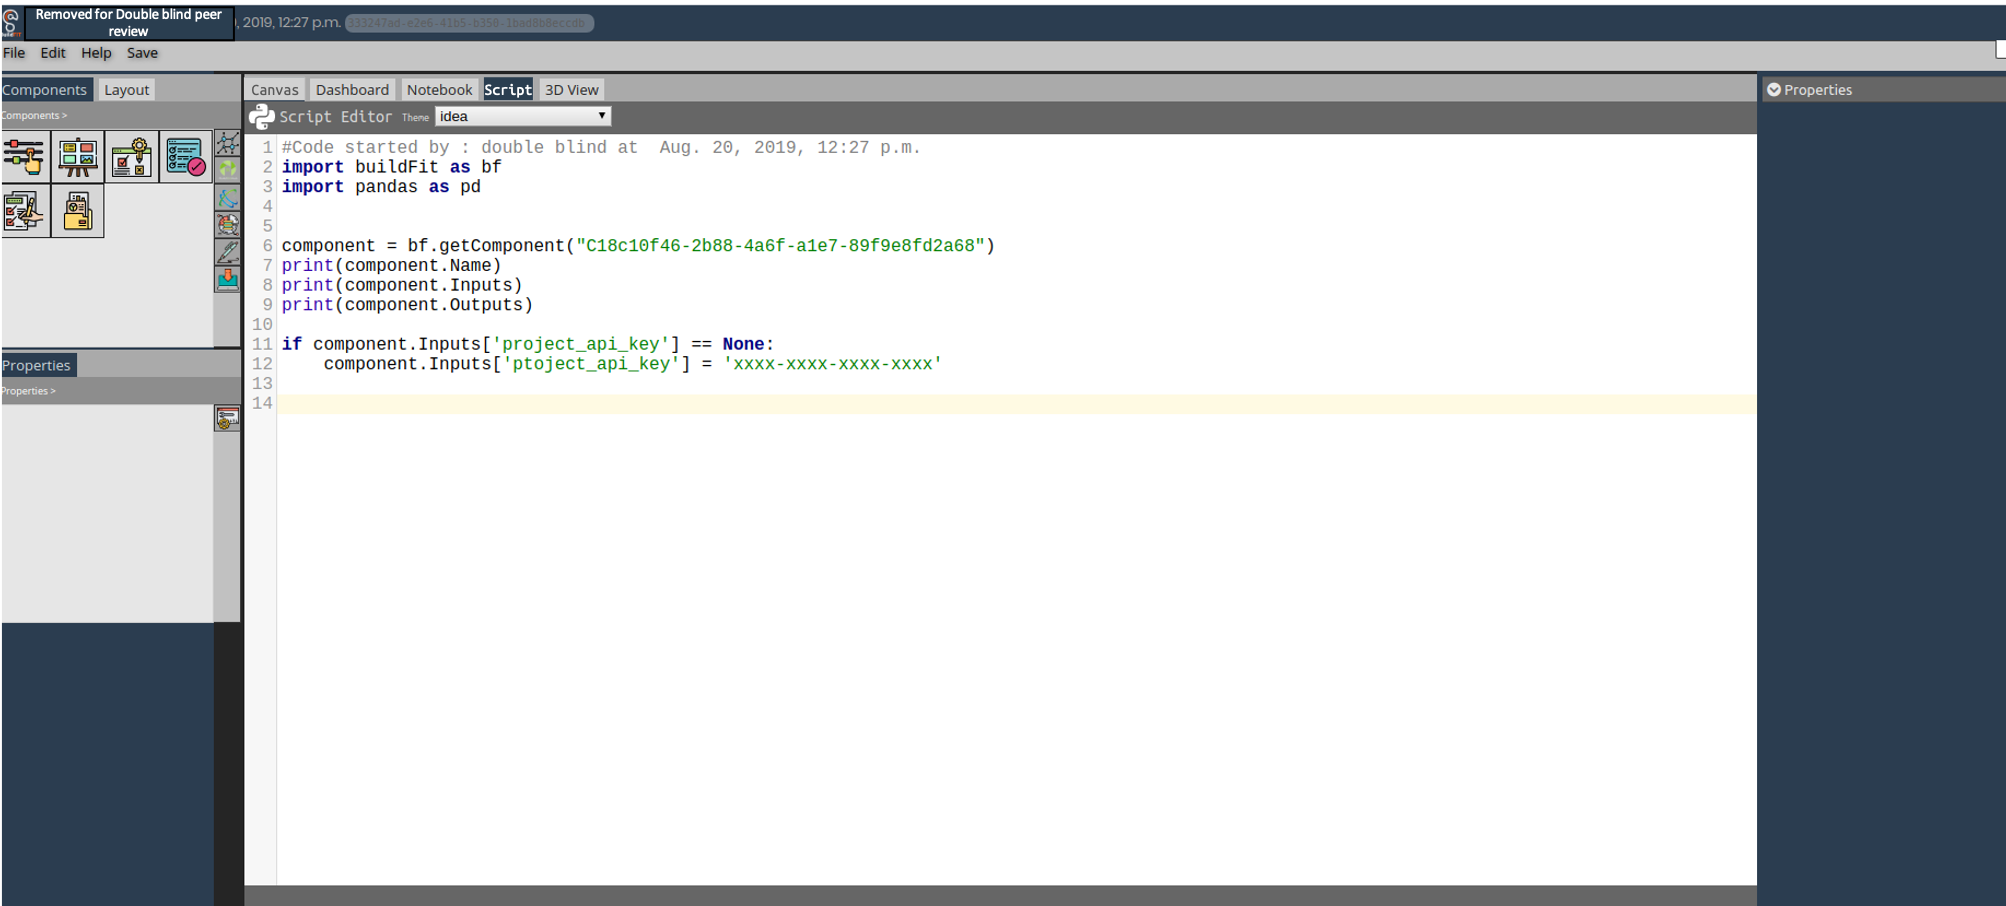
\includegraphics[width=\columnwidth]{imgs/tpl_interface.png}
\caption{TPL interface using Python script. The python script enables reading, writing inputs and outputs of different components, as well as adding pre/post processing functions to the inputs/outputs.}
\label{fig:tpl_interface}
\end{figure}
\subsection{Dashboard and forms}

\label{sec:applicationlayer}
The dashboard and forms are located in the same tab called 'Dashboard'. It is an information management tool directed to stakeholders who are not involved directly in the development of the project i.e., to track performance, metrics, and other key data points; or to get feedback and other user inputs (questionnaires or thermal comfort feedback). The project owner does the design of the dashboard, using the input components (e.g., numeric slider, optionList, listView, RadioButtons, and  Panels ) and the output components (e.g., Panels, Plots, 3D views, 2D plans, images, videos etc.). Then, the dashboard could be shared with public or specific people to view or interact. It can also be embedded within other websites.
\section{Application Layer}
The application layer receives the deep function requests from the presentation layer in the form of a JSON object following specific schema. On the one hand, If there are data-related processes, it sends a request to the data layer (explained in detail in section \ref{sec:datalayer}. On the other hand, if there are no database-related processes, the JSON object consisted of the inputs and the component function callback. The function then starts to operate in three cases:
\begin{enumerate}
    \item It runs the function directly from the node. 
    \item It starts other cloud engines to run the functions. 
    \item It uses third party engines (e.g. BuildSimHub) to perform the operation. 
\end{enumerate}
Consequently, the function response back to the presentation layer as a JSON object with the outputs (if any), Errors, and logs. The response JSON object also follows a predefined schema as shown in figure \ref{fig:component}. The whole process is illustrated in figure \ref{fig:structure} (steps: 1, 2, 3, 8, 9).


\section{Data Layer}\label{sec:datalayer}

There are four major types of data involved in this platform: metadata of the users and projects, metadata of the buildings, building models, and building operational data. The data layer has three main functions: \textbf{Data querying}: to acquire data from multiple data sources, \textbf{Data storage}: to store different types of data, and \textbf{Data feed}: to respond to the requests from the application layer.\par

The metadata and models are either input by the users through the presentation layer or assigned by the application layer. These data are mainly text. Once passed to the data layer, they are static and stored in the relational databases (Figure \ref{fig:relationDatabase}). As for the building operational data, the time series data comes from servers of different Building Management Systems. BMS in different buildings are various, in terms of data structure, sampling rate, communication protocol, etc., making data querying a troublesome task. The platform dealt with this by deploying the PI system from OSIsoft, which queries data from different types of servers, such as BACnet (Building Automation and Control networks) and OPC (Open Platform Communications), and stores the compressed data on the local server.\par
\begin{figure}
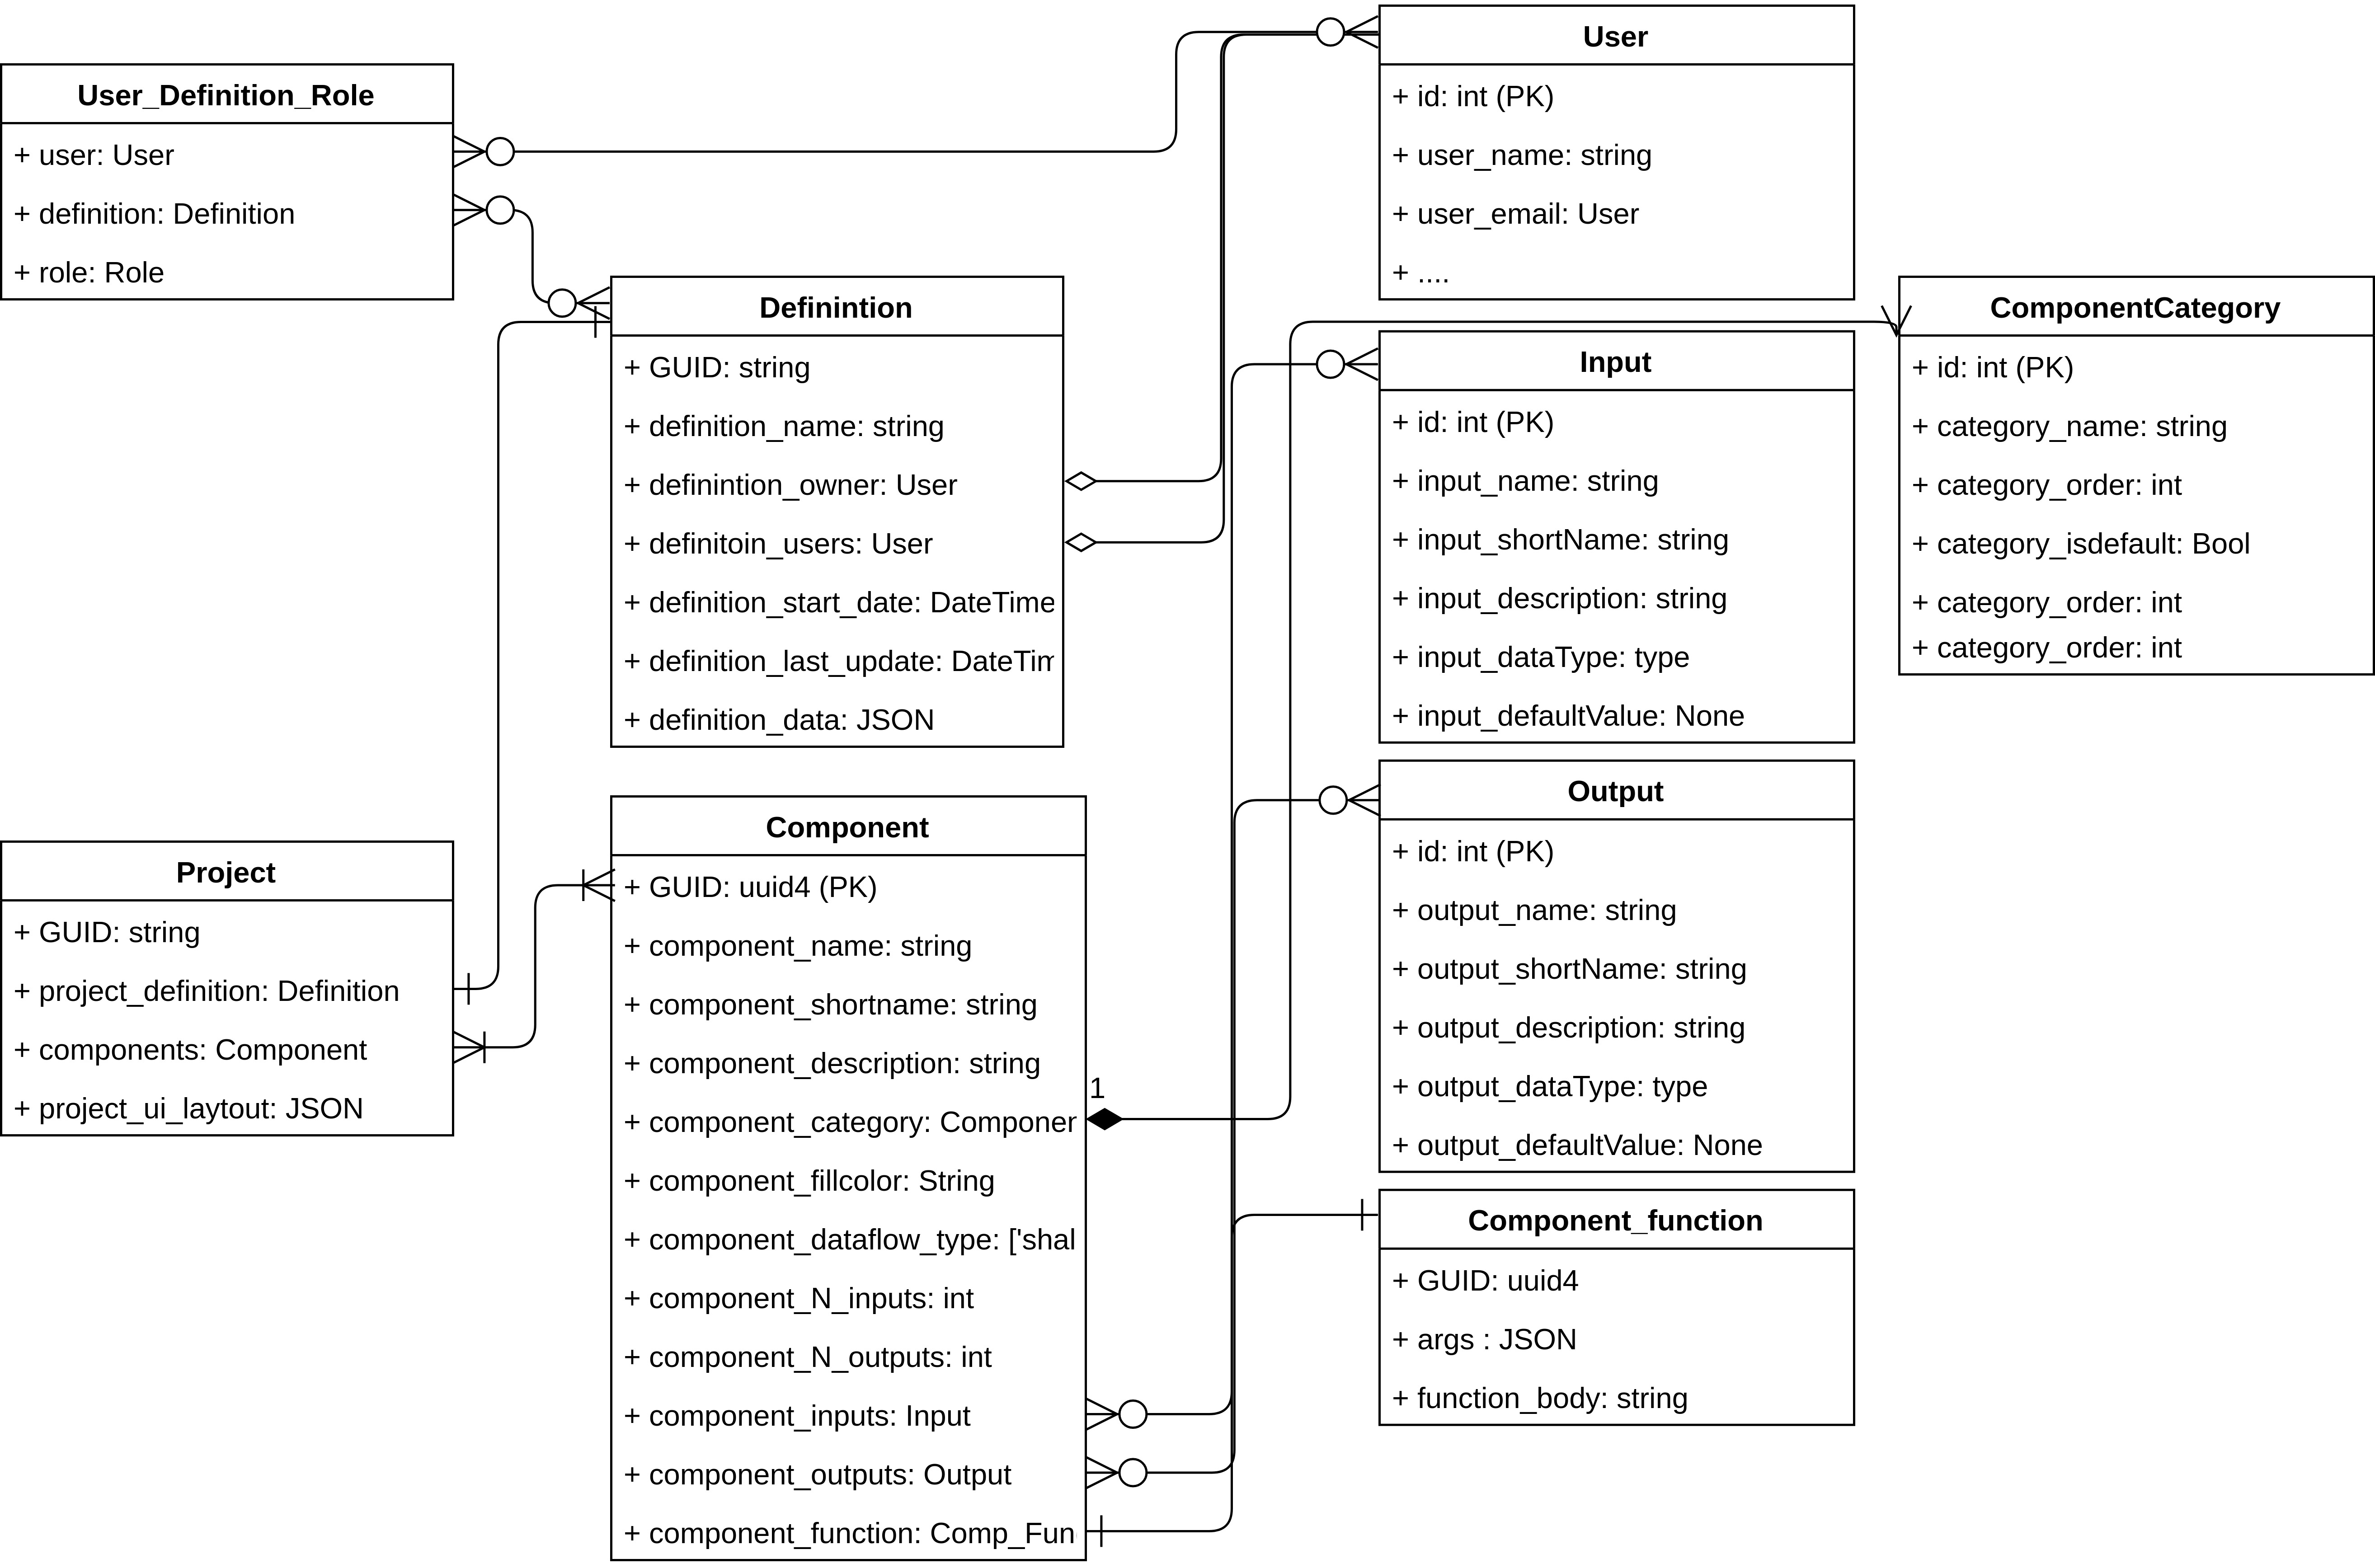
\includegraphics[width=\columnwidth]{imgs/uml_relationship.jpeg}
\caption{Relational database: A higher resolution image can be downloaded  \href{https://user-images.githubusercontent.com/6969514/72235771-e9e89f80-360e-11ea-9cf7-91c0f521576c.jpeg}{here}. 
}
\label{fig:relationDatabase}
\end{figure}
Data exchange between the application layer and the data layer is done through RESTful API and mainly in JSON format. For example, if a user wants to see the energy consumption trend of a building, he/she will select the data point and define the time period in VPL canvas. The deep functions in the application layer will get the information and accordingly send the request. The API will retrieve data from the server and send it back as a JSON file, which will then be plotted in the canvas.

\section{Use case scenario} \label{section:casestudy}
In this section, we introduce a use case based on Cockburn's template \cite{Cockburn1998UseTemplate}  to illustrate how the platform works. The use case is a parametric energy simulation of a small office building from ANSI/ASHRAE/IES Standard 90.1 commercial reference buildings \cite{Field2010UsingStudies} shown in figure \ref{fig:commrefbuild}.

\begin{figure}[h]
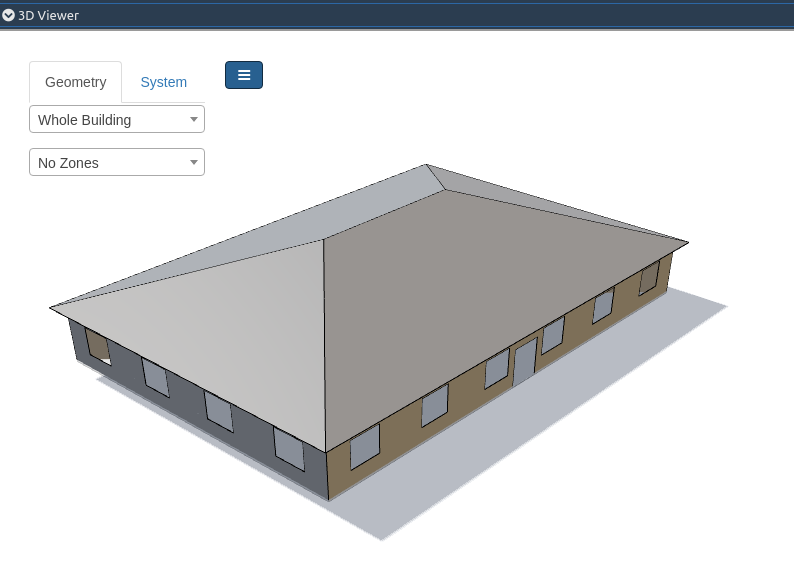
\includegraphics[width=\columnwidth]{paper_LateX/imgs/comm_ref_build.png}
\caption{One of the reference buildings developed by the U.S. Department of Energy (DOE). The building represents a small office with 5,500 square feet area and one floor. The image is a screenshot taken from the embedded 3d viewer in our platform, and provided by BuildSimHub (in the application layer). an animated GIF of the 3d-viewer could be viewed \href{https://user-images.githubusercontent.com/6969514/77833696-3eb1a600-717a-11ea-8f77-475be6d57cfb.gif}{here}}
\label{fig:commrefbuild}
\end{figure}
\textbf{USE CASE:1 Conduct a Parametric Energy Simulation}\\
- - - - - - - - - - - - - - - - - - - - - - - - - - - \\
CHARACTERISTIC INFORMATION\\
\textbf{\underline{Context of use:}} EnergyModeller conducts a parametric building energy simulation of a small office building using the three-tier architecture platform.\\
\textbf{\underline{Scope:}} Platform\\
\textbf{\underline{Level:}} Summary\\
\textbf{\underline{Preconditions:}} The user must have a valid authentication to the platform and a supported web browser (e.g. Google Chrome).\\
\textbf{\underline{Actor(s):}} EnergyModeller, BuildSimHub (cloud simulation engine).\\
\textbf{\underline{Trigger:}} Firstly, the EnergyModeller should start a new project. Secondly, IDF file of the EnergyPlus model of version greater than 8.0.

\underline{Description: }
\begin{enumerate}
    \item EnergyModeller starts a new definition (project).
    \item The IDF file link and global unique id (GUID) are retrieved. 
    \item EnergyModeller uploads the IDF file to the data layer (a scalable google cloud bucket) using a file upload component (Figure \ref{fig:fileupload_comp}) -- an animated GIF image could be viewed \href{https://user-images.githubusercontent.com/6969514/77833649-16c24280-717a-11ea-9df1-8a5e0f7bae83.gif}{here}.
    
    \item EnergyModeller loads a "buildSimHub Parametric Study" component (Figure \ref{fig:parametric_study}). 
    \item fsdfsafasdf
    \item fsdfsafasdf
    \item fsdfsafasdf
\end{enumerate}

\begin{figure}[h]
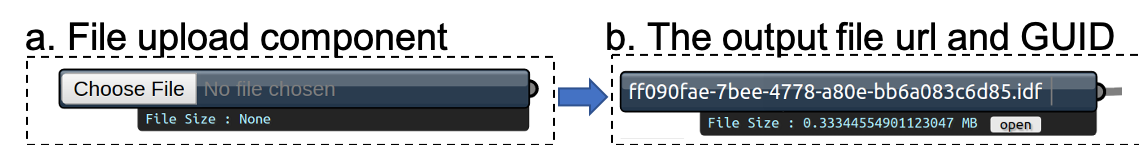
\includegraphics[width=\columnwidth]{paper_LateX/imgs/file_compo.png}
\caption{ File upload component in the presentation layer: a) The user is prompted to select a file. The file is uploaded to a google cloud bucket; b) Then, the file could be triggered by its global unique id}
\label{fig:fileupload_comp}
\end{figure}

\section{Conclusion}
In this paper, we explained an approach for applying Client/Server based architecture called 3-tier architecture (summarized in figure \ref{fig:structure}). This approach is used for managing data from the built environment using a cloud-based user-friendly visual programming interface. This approach depends on separating the client-side (called the presentation layer) from the back-end engines (the application layer) and the databases (the data layer). This separation eased the distribution of computation power over many nodes without compromising the efficiency of the other layers. Furthermore, it overcame some problems related to latency and connection speed. Moreover, flexibility and scalability are two key features of this type of architecture. 

Future development includes enabling real-time teamwork, version controls, besides continuous testing and user-experience improvements. 

\section*{ACKNOWLEDGMENTS}
% This paper is a part of a project funded by the Ng Teng Fong Charitable Foundation (NTFCF) research funding.
% \clearpage
% \balance



\bibliographystyle{scsBiblioStyle}

\bibliography{references.bib,references2.bib}
\end{document}
